\chapter{Methods}\label{ch:methods}
Let us continue by estimating conservatively on how much data is produced when using the LAMP end-station with both pnCCD detectors in use at a $120$hz. Each pnCCD produces 120 images per second, each image is in a 32 bit per pixel format such that an image is vaguely $4$megabyte in size. So, every minute, the front \& rear pnCCD produce approximately $60$ gigabyte of data. To analyze these vasts amount of data an extensive set of methods and optimized algorithms is required. This chapter is devoted to the analysis methods used in the present thesis.\\
The chapter is organized as follows, section \ref{sec:LCLS-computing} describes the general LCLS computing environment to establish an overview of the hard- and software capabilities. Section \ref{sec:pnccd-corr} discusses corrections that are applied to the raw pnCCD images. In section \ref{sec:hitfinding}, several hitfinding methods are being evaluated. Finally, section \ref{sec:phase-retrieval} goes over used phase-retrieval algorithms.
%
%
%
\section{The computing environment at LCLS}\label{sec:LCLS-computing}
%%%%%%%%%%%%%%%%
%- Include basics around the PSANA interface\\
%- For example how the date is converted, then stored and\\
%- the analysis opportunities along the way
%- I think this will be a longer subsection since a lot of my work went into this and I'm regularly contacted about it.
%- Short introduction what we have to go through\\
%- Reminder of detectors and analysis environment
%%%%%%%%%%%%%%%%
\begin{figure}
	\centering
		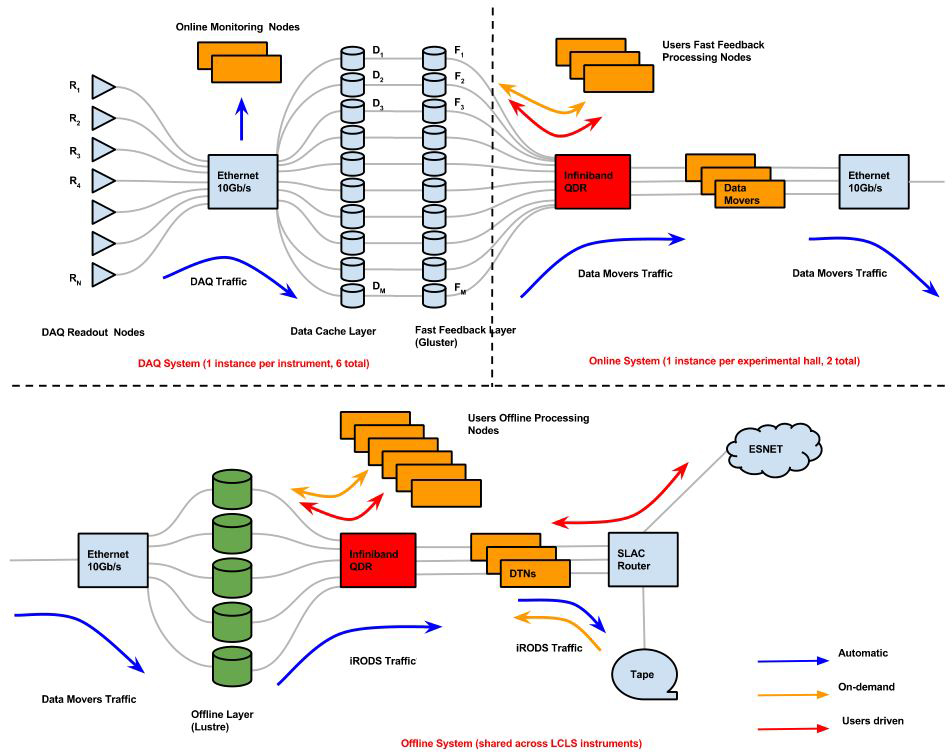
\includegraphics[width=1.00\textwidth]{images/daq-architecture.JPG}
	\caption{caption. From \citep{Amadeo-2016-SLAC}}
	\label{fig:daq-architecture}
\end{figure}
As estimated above, the vast amounts of data generated by LCLS are unhandy for a single group of visiting scientists that perform experiments there. For this reason the LCLS data acquisition (DAQ) group has incorporated many detectors, for example the the pnCCD and Aqciris digitizer into their framework. All data taken at LCLS is stored in the LCLS computing environment, where the data can also be analyzed. As indicated in figure \ref{fig:daq-architecture}, DAQ readout nodes send the data traffic via ethernet to a short-term cache and fast feedback (FFB) layer. While the data is being transferred, online monitoring nodes are able to 'see' a fraction of the live (online) data and run analysis. With a delay of a few ten seconds, the FFB nodes can be used to run analysis on the full data stream with, thereby having 'online' and 'offline' data access and more computing power process all data. Eventually the data is being moved to the 'offline' layer, where the data is managed by the integrated Rule-Oriented Data System (iRODS). The data is stored in .XTC file containers and it can also be accessed from outside SLAC (Router \& ESNET). The stored data has certain storage quotas and times. In brief, there is a 6 months short-term storage without quota limitations and a two-year medium-term storage with a storage quota of $10 000$ Giga-Byte. After that, the data is automatically stored for at least 10 years on magnetic tape (long-term storage) and can be restored upon request. A web interface is provided by the DAQ group to simplify and automate the data-handling and logging process. The short- and medium term storage solutions can also be used to analyze the data using the psana-framework to access data and allows computation on the psana computer cluster with over 1000 CPU cores. The psana-framework can be interacted with using python 2.7. The interacting python script calls functions within the psana-framework that are programmed in C(++), for example detector calibrations. Psana allows parallelization via MPI and it is therefore possible to analyze many events (LCLS pulses) simultaneously. Also complex analysis is able process at the rate of the incoming data using MPI, when the FFB is used. Python scripts can be written for 'online' or 'offline' analysis and are fairly similar.\\
For LCLS-II, this analysis and data-access scheme is designed to be similar \citep{Amadeo-2016-SLAC} with the exception of the online monitoring nodes. It is therefore recommended to build analysis schemes that are based on the FFB, which can then be used later as offline analysis as well. A quick introduction on how to use psana can be found in the appendix \ref{sec:python-example}, where a few examples from the LCLS DAQ group are condensed.
%
%
%
\section{pnCCD photon detectors}\label{sec:pnccd-corr}
%%%%%%%%%%%%%%%%
%- Describe signal on the pnCCDs\\
%- Calibrations and corrections - use LAMP paper\\
%- single hits\\
%- multiple hits
%%%%%%%%%%%%%%%%
\begin{figure}
	\centering
		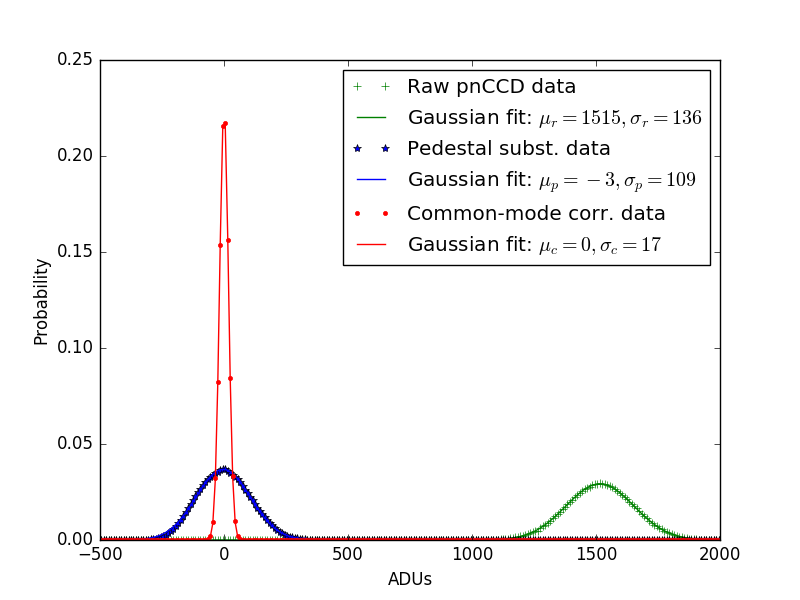
\includegraphics[width=1.00\textwidth]{images/pnCCD-electronic-noise.png}
	\caption{caption}
	\label{fig:pnCCD-electronic-noise}
\end{figure}
Before the pnCCD detectors can be used to take data, it is good practice to apply corrections to the raw detector image in order to cope with electronic noise. Since these corrections are used often, the LCLS detector and DAQ group has implemented a calibration manager tool\index{psana!calibman}\footnote{The calibration manager tool 'calibman' can be found in the 'psana' software package. More information under \url{https://confluence.slac.stanford.edu/display/PSDM/Calibration+Management+Tool} (Oct 2016)} that provides the algorithms necessary and helps with the procedure of applying image corrections and more. We discuss the two most often used corrections next. One, corrects for the electronic noise pedestals\index{pnCCD!pedestal correction} (levels) of each pixel, and two, accounts for common modes\index{pnCCD!common mode}, e.g. artifacts from the read-out electronics.\\
%
We illustrate the effects of applying these corrections in figure \ref{fig:pnCCD-electronic-noise} through a set of histograms. The histogram bins are showing ADU values from dark pnCCD images in highest gain. The green curve shows the ADU values of a raw detector image where no corrections have been applied, i.e. the electronic noise response from the chip has a standard deviation of $\sigma_{r}=136$. Note, that there is also a significant offset of the distribution from the 0 to $\mu_{r}=1515$ ADU. The blue curve shows the same data but is using the pedestal corrections found in 'calibman'. The pedestal corrections reduce the noise slightly to $\sigma_{p}=109$ ADU, and as expected, the pedestal corrections drastically move the normal distribution to be centered around $\mu_{p}=-3$. Finally, the red curve is also the same data than the green curve but includes pedestal and common-mode corrections. The corrected read-out modes drastically improve the standard deviation to $\sigma_{c}=17$ and slightly move the mean to $\mu_{c}=0$.\\
As a guideline, the pedestal corrections should be always used to account for the mean offset. The common-mode calibration, however, should be tested before applying. The algorithm that determines common-modes needs to find a baseline and therefore needs pixel with no signal. To give an example where no common-mode corrections should be applied, it is sometimes the case in single-particle imaging that the detector is illuminated in (almost) every pixel. Then the common-mode correction algorithm may treat real signal as noise and fail to find a common baseline.\\
%
%
%
%\subsection{Signal analysis}
%- Present data from 1500eV photon energy on Xe backfilled chamber with the pnCCDs in spectroscopy mode to argue that the pedestal and offset corrections are enough to correct for fluoresence.\\
%- Masked areas in image
%%%
%
%
%
\subsection{Combining multiple pnCCD detectors}\label{sec:combination-of-images}
%%%%%%%%%%%%%%%%%%%%%%%%%
%- Explain how I combined pnCCD detectors to perform reconstructions on it.\\
%- Can reuse material from the LAMP pnCCD paper
%%%%%%%%%%%%%%%%%%%%%%%%%
In order to maximize resolution, it is most useful to combine multiple pnCCD detector modules into one image. In theory, this is an easy task. One combines the detectors using scattering vector and some reference objects to align the system. While it is simple for the human eye to merely combine the diffraction patterns, it is a more complex task to actually prepare the combined images for phase-retrieval algorithms that use fast Fourier transformations (FFTs). In fact, it has not yet been shown in single-particle imaging that it is possible to retrieve a real space image from multiple detectors in different planes. One of the reasons is, that the samples that were studied in recent years were comparably large, e.g. viral samples of a few hundred nanometre radius that don't scatter to wide angles. Therefore, in many experimental setups, the distance of this detector is then set to fill the detector planes appropriately to the scattering of the sample. In other words, there was no incentive of combining detectors. With the intensities provided by LCLS and the single-particle imaging capabilities of the LAMP end-station, we can now study objects that are smaller than a hundred nanometre in radius but are still able to study larger samples. To cover this variety in object size, LAMP's front pnCCD detector can move along the z-axis and can cover wide scattering angles from smaller objects and LAMP's rear pnCCD detector covers the usual small angles scattering from larger objects. Once the detector is set to cover most scattering angles, one finds that the dynamic range and photon sensitivity becomes a limiting element. This is where combining multiple detectors gets very attractive, because they can be operated in different gains but still be combined efficiently. Summarising, the combination of multiple detectors gives the ability to cover large scattering angles while increasing the dynamic range.\\
Let us now describe the process of combining diffraction images while simultaneously preparing them for the inverse problem of phase-retrieval. It is first best to express the dispersive scattering process using the scattering vector $\vec{q}$ as
\begin{equation}
\vec{q} = 4 \pi \frac{\sin\left(\frac{\Theta}{2}\right)}{\lambda},
\label{eqn:q-vector}
\end{equation}
with $\vec{q}$ being the scattering vector, and $\lambda$ being the wavelength of the scattered photons. Through careful alignment and calibration, we can now map a scattering vector $\vec{q}$ to each pixel. Using this information, we project the pixel onto a single plane, e.g. we used the front plane in this work, and combine the pnCCD modules. At this point, we want to emphasise that the the alignment of the overlapping pnCCDs matters much. We found that even slight miss alignments of 2-3 pixel in the digital detector plane result in unphysical effects in the real-space image. Projecting the pnCCD detectors onto one plane changes the effective pixel sizes. However, in order to use Fast Fourier Transformation (FFT) algorithms that are often used to solve the inverse problem, one needs to keep the pixel size the same. In our case, we down-sample the rear pnCCD choosing the down-sampled pixel size to match the front pnCCD size, thereby, adding the average intensity values in the down-sampled pixel. To be in compliance with the FFT algorithms, one should also fill the gaps left and right of the rear pnCCD projection with zero value pixel. After the alignment of the pixel, we need to adjust for the different gains and detector distances. As described above, the ADU value creation is well specified in the pnCCDs and we can use the gain factors to normalise the ADUs. We must then adjust the intensity levels for their relative position to each other by a factor of $\frac{d_{rear}^{2}}{d_{front}^{2}}$, with $d_{rear}$ being the distance from the IR to the rear pnCCD and $d_{front}$ being the distance from the IR to the front pnCCD.\\
\begin{figure}
	\centering
		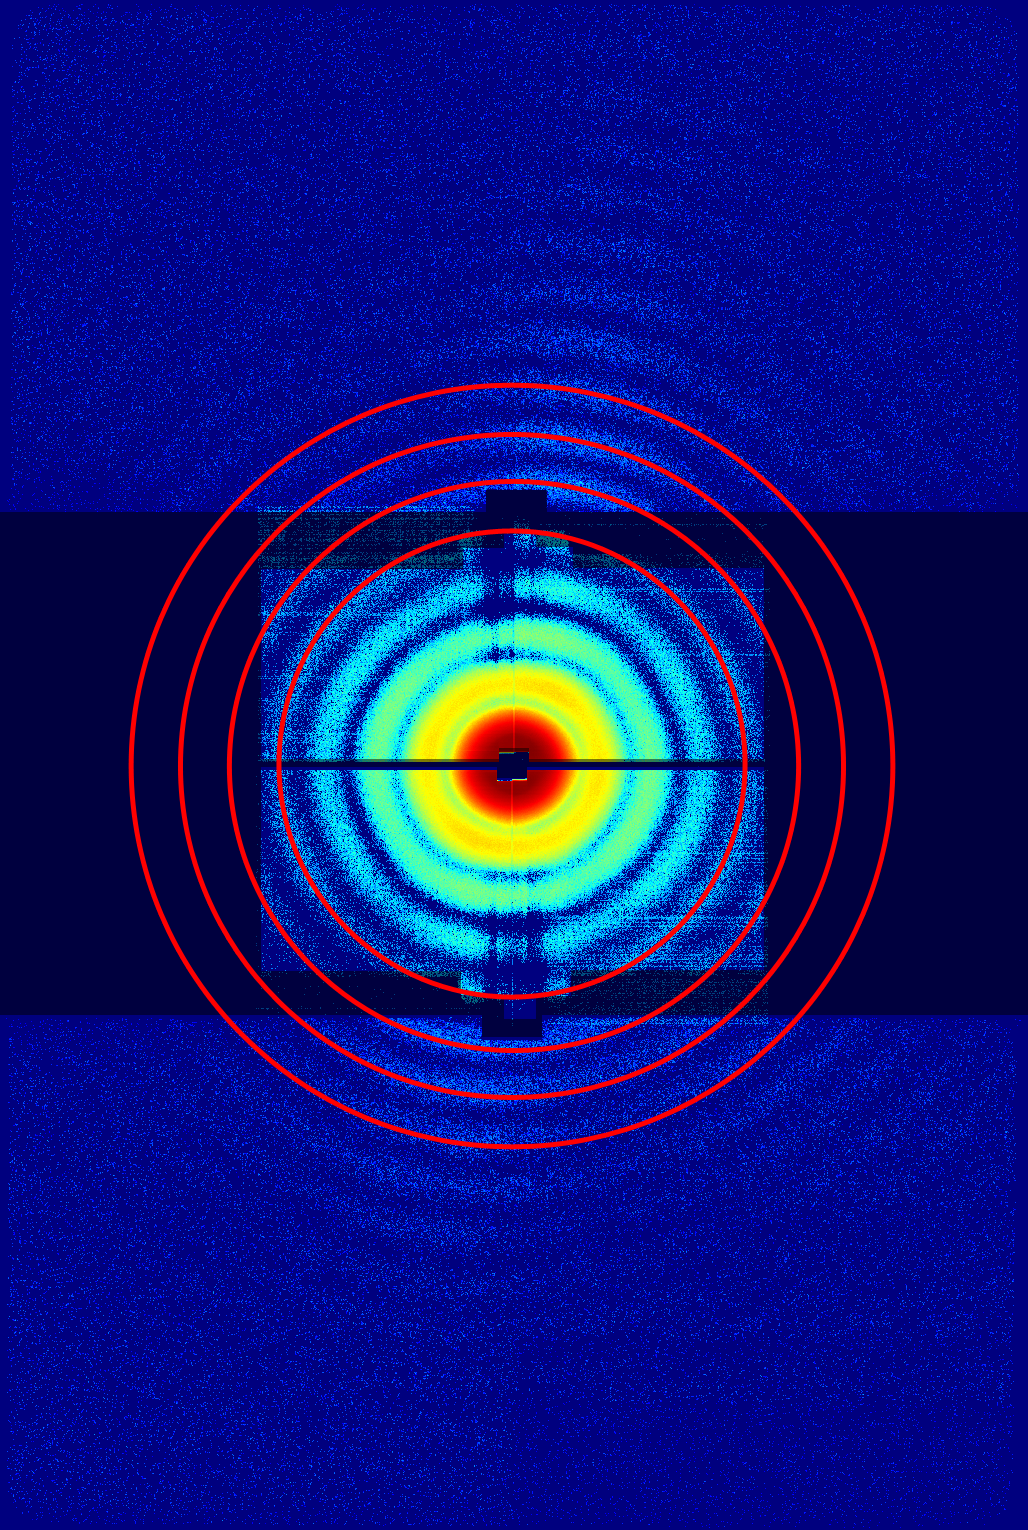
\includegraphics[width=0.80\textwidth]{images/pnCCD-image-geometry.png}
	\caption{A combined pnCCD image using the full image of the front pnCCD and a down-sampled image of the rear pnCCD. The red circles in the image are drawn in to visualize the alignment of the detectors. As described in the text, the intensities in the image are normalized and corrected for different electronic gains and distance to specific detectors. The shaded areas are not covered by the pnCCDs and are therefore masked out.}
	\label{fig:pnCCD-image-geometry}
\end{figure}
Figure \ref{fig:pnCCD-image-geometry}a shows a diffraction pattern from a spherical xenon cluster of ~$50$ nm in radius. The front pnCCD detector was set to slightly overlap with the rear pnCCD detector along the y-axis but the front detector was set $~365$ mm closer to the interaction region along the z-axis. All four of LAMP's pnCCD planes have been combined in one image, and since the rear pnCCD is farther away from the interaction region it appears smaller on the combined image. The red circles are a help to align the detectors and show how the diffraction pattern overlaps from one detector module to another. In this case, the front pnCCD was operated in highest gain $\frac{1}{1}$ and the rear pnCCD was operated in lowest gain $\frac{1}{256}$.\\
\begin{figure}
	\centering
		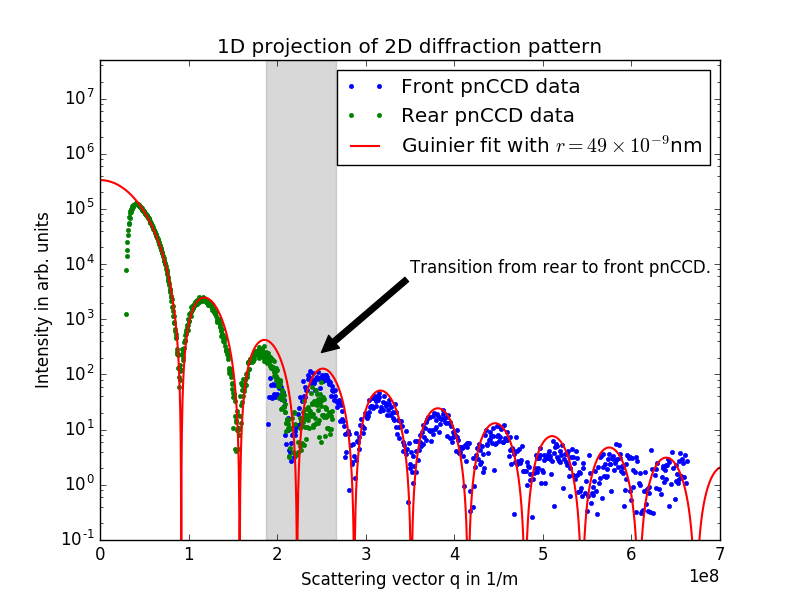
\includegraphics[height=0.50\textwidth]{images/pnCCD-1d-sum.png}
	\caption{In this graph a 2D diffraction image was projected onto 1D assuming a spherical symmetry of the diffraction pattern. The green data points are gathered from the rear pnCCD and the front pnCCD data points are reflected by the blue data points. The red curve is a simulated scattering curve from an ideal sphere that has a radius of $49 nm$. The amplitude of the red curve has been fitted to the data points and it agrees well with the data over 8 diffraction rings. The gray shaded area shows the transition area from rear to front detector.}
	\label{fig:pnCCD-1d-sum}
\end{figure}
At this point, the radial intensity profile yields valuable information about the geometric alignment and intensity normalization. Figure \ref{fig:pnCCD-1d-sum} shows the radial intensity profile of the spherical symmetric diffraction image over 5 orders of magnitude above the noise level. The red curve illustrates the expected scattering intensity of a spherical object with radius $49$nm and the amplitude was fitted onto the rear pnCCD data. The curve showcases the validity of the detected signal up to the edges of the front pnCCD, where a lack of signal is prevailing. There are also some discrepancies from the red curve on the transition from the rear to front pnCCD, which are due to the shade projected from the front onto the rear pnCCD and the resulting lack of signal.
%
%
%
\subsection{Impact of X-ray pump -- X-ray probe on diffraction pattern}
\begin{figure}
	\centering
		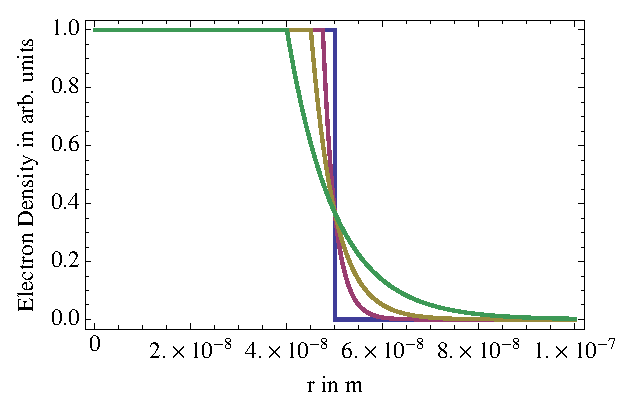
\includegraphics[width=0.49\textwidth]{images/electron-density-convoluted-object.eps}
		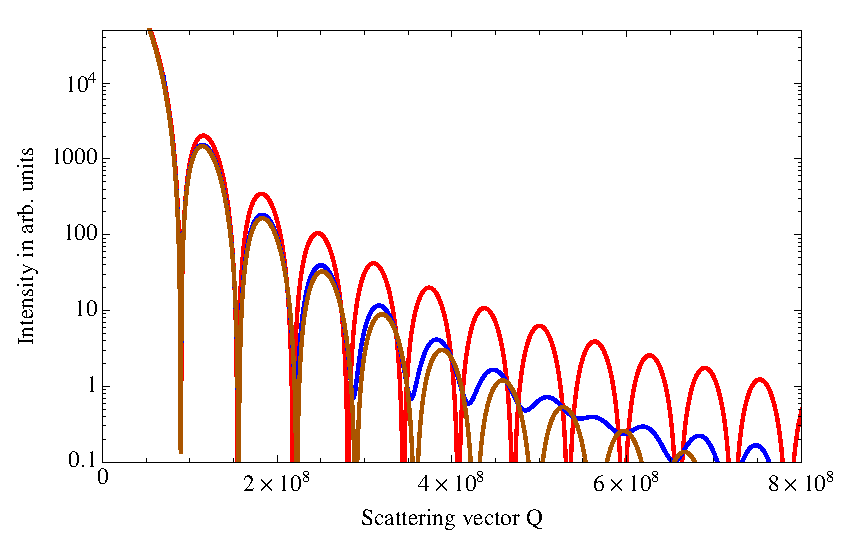
\includegraphics[width=0.49\textwidth]{images/beam-convoluted-with-object.eps}
	\caption{caption}
	\label{fig:electron-density-convoluted-object}
\end{figure}
In a coherent diffractive imaging X-ray pump -- X-ray probe experiment, both pulses contribute to the scattering image. The pump pulse will project an image of the solid and intact cluster, while the probe pulse will propagate an image of the expanding, damaged cluster. In the present experiment, the pump pulse was set at $\sim10\%$ of the overall pulse energy, while the probe pulse was set to $\sim90\%$ of the overall pulse energy. In order to simulate the effects of this pump--probe setup, a 1D simulation is conducted using electron densities $\rho\left(r\right)$ of spheres. The spheres are allowed to expand after the model
\begin{align}
\rho\left(r, k\right)&=\begin{cases}
1& \text{for $R-k \geq r \geq 0$},\\
e^{\frac{(R-k)-r}{k}}&\text{for $R > r - k$},
\end{cases}
\intertext{with $R$ being the cluster radius and $k$ an expansion coefficient such that}
\int_{0}^{\infty}\rho\left(r, k\right)dr &= R,\quad \text{if } 0<k<R 
\label{eq:el-density}
\end{align}
The electron density can then be Fourier transformed into recipocal space using the transformation \citep{Guinier-1955-JWS}
\begin{equation}
F^{2}(Q)=A\left(\int_{0}^{\infty}\rho\left(r,k\right)\frac{\sin\left(Q r\right)}{Qr}4 \pi r^{2}dr\right)^{2},
\label{eq:guinier-fourier-transform}
\end{equation}
with $A$ being an intensity scaling factor. The electron densities for $R=50$ nm and $k=\{0,2.5,5,10\}$ nm are shown in figure \ref{fig:electron-density-convoluted-object} left. Figure \ref{fig:electron-density-convoluted-object} right showcases several cases of the (expanding) sphere in reciprocal space. The red line is the scattering of a solid sphere $F_{\text{undamaged}}^{2}$, with $A$ being used to scale the intensity to typical experimental data. The brown curve is the scattering of a damaged sphere $F_{\text{damaged}}^{2}$ with $R=50$ nm and $k=5$ nm. Lastly, the blue curve corresponds to the case, where $A\cdot F^{2}\rightarrow A \cdot 10\% F_{undamaged}^{2}+A \cdot 90\% F_{damaged}^{2}$. Although the pump pulse influences the diffraction pattern visibly at high-Q values, the added signal remains in the noise level of $F^{2}<1$ (compare figure \ref{fig:pnCCD-1d-sum}).
%
%
%
\section{Data filtering}\label{sec:hitfinding}
%%%%%%%%%%%%
%- Discuss the hitfinding.\\
%- iTOF vs. pnCCD\\
%- vs. Actual dynamics visible in diffraction images
%%%%%%%%%%%%
\begin{figure}
	\centering
		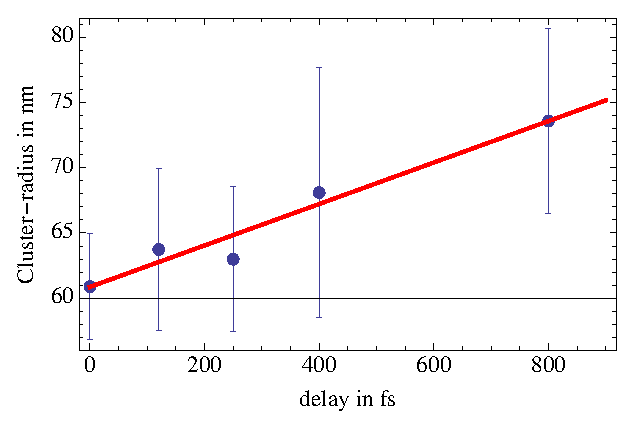
\includegraphics[width=0.49\textwidth]{images/filter-size.eps}
		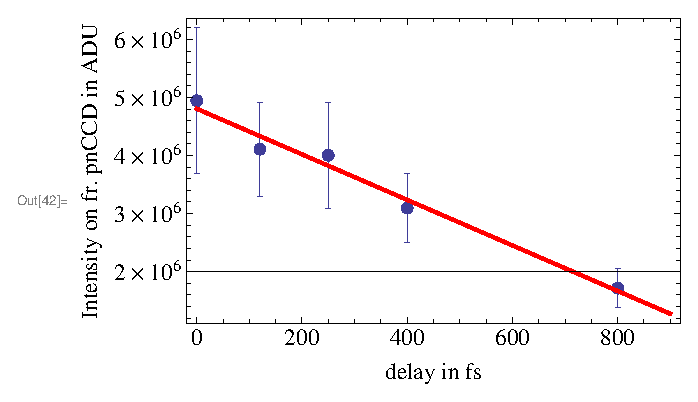
\includegraphics[width=0.49\textwidth]{images/filter-sum-frontpnCCD.eps}
	\caption{caption}
	\label{fig:filter-size-intensity}
\end{figure}
As described in the above sections, LCLS produces large amounts of data. This data has to be filtered to a point, where it can be used for phase retrieval. The coincident detection of diffraction image and time of flight spectroscopy allow great freedom to filter on useful events. For the present work, a useful event is the interaction of X-ray pump -- X-ray probe with a single cluster system. On the one hand, cluster produce the most intense signal on pnCCD and TOF detectors when they are in the center of the intensity profile of the LCLS beam \citep{Gorkhover-2012-PRL}. On the other hand, as the time delay $\delta t$ of the X-ray pump -- X-ray probe is increased, the nanoplasma expansion leads to a decrease in signal on the pnCCD (see figure \ref{fig:filter-size-intensity}). This can be extrapolated to an extreme, where cluster would not produce any signal on the front pnCCD. In order to filter on the full bandwidth of interesting hits, a series of filters have been applied. Filtering on ion time of flight high charge states states has been successful in overall gathering images resolving pump--probe dynamics. In figure \ref{fig:filter-size-intensity} left, the xenon pump--probe data has been autocratically pre-filtered on high-charge states, leaving several thousand events that were then manually reduced to over 350 single-hit diffraction images. These events indicate a linear average cluster radius increase of $\sim15\%$ over the course of the first 800 fs at a given pump pulse energy. The size determinations have been performed using the first maxima as described (see section \ref{TBD}). However, to perform phase retrieval and to solve the inverse problem, bright hits containing many photons are required. Therefore, an additional hitfinder on a snippet of the rear pnCCD detector has been implemented. It determines the scattering intensity in single hits. 
%
%
%
\section{Phase retrieval from a single diffraction pattern}\label{sec:phase-retrieval}
%%%%%%%%%%%%%%
%- Short intro into phase retrieval
%%%%%%%%%%%%%%
As deducted in section \ref{sec:saxs}, coherent diffractive imaging merely measures the intensity in reciprocal space and the phase information, i.e. complex fields, are lost. The scattered intensity $I\left(\vec{Q}\right)$ is proportional to the form factors $\left|f^{0}\right|^{2}$. Iterative algorithms can retrieve this lost information because there are only limited sets of phases that uniquely reproduce the diffraction image \citep{Bruck-1979-OpticsCom,Bates-1981-Optik}. To fully recover the original function, i.e. real and complex values of the diffraction pattern, the diffraction image must be oversampled \citep{Sayre-1952-ActCryst}. Here, the Nyquist-Shannon sampling theorem says that an Fourier transformed object of size $X$ can be fully recovered if its sampling rate is at the Nyquist rate of $\frac{1}{2X}$. The Nyquist rate can be translated into a minimum (pnCCD) pixelsize in realspace using the following relation between a discrete Fourier transform and pixel size \citep{Williams-2010-NJP}
\begin{equation}
\Delta_{r} = \frac{\lambda L}{2 X},
\label{eq:disc-fourier-relation-pixelsize}
\end{equation}
with the wavelength $\lambda$, the length to the detector $L$ and the object length along one dimension $X$. For typical experimental values, the sampling pixel size must be $\Delta_{r} = 2.7$ mm. The pnCCD pixel size of $75 \times 75~\mu\text{m}^{2}$ samples the object sufficiently enough.
%
%
%
\subsection{The inverse problem: Phase retrieval}
%%%%%%%%%%%%%%
%- Introduce some aspects from phase retrieval algorithms.
%%%%%%%%%%%%%%
\begin{figure}
	\centering
		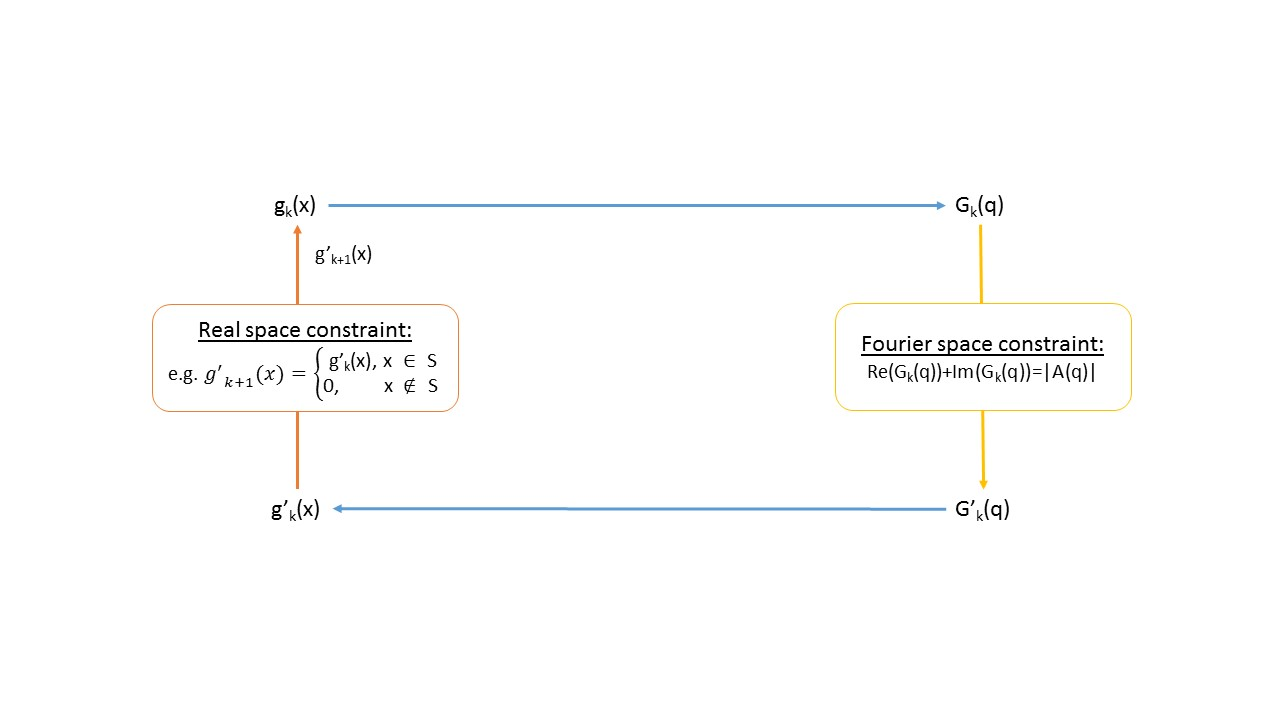
\includegraphics[width=1.00\textwidth]{images/phase-retrieval-algorithm.jpg}
	\caption[Example of a phase retrieval algorithm.]{Principle of a phase retrieval algorithm. The real space object $g_{k}\left(x\right)$ is Fourier transformed to $G_{k}\left(q\right)$. The function $G_{k}\left(q\right)$ is altered to fit the constraints set in Fourier space, hence $G'_{k}\left(q\right)$. $G'_{k}\left(q\right)$ is inverse Fourier transformed to $g'_{k}\left(x\right)$. After fulfilling the real space constraints the iterative starts again using $g_{k+1}\left(x\right)$. From \citep{Fienup-1982-AO}.}
	\label{fig:phase-retrieval-algorithm}
\end{figure}
To recover the phase and thus reconstruct the particle iterative algorithms have been developed \cite{Fienup-1982-AO}. Figure \ref{fig:phase-retrieval-algorithm} illustrates such an iterative algorithm, where the image of an object $g_{k}\left(x\right)$ is Fourier transformed to reciprocal space $G_{k}\left(x\right)$ and then back again resulting in $g_{k+1}(x)$, while sufficing certain constraints.\\
The constraints are rather strict defined in the reciprocal space as they have to reproduce the actual measurement $I=A\cdot A^{*}$. The criteria that need to be met in real space can be chosen more freely. Generally, the recovered object should be physical, i.e. consist of positive values or should be of a certain (known) size. In simplified terms, one can introduce a support structure $S$ that meets the physical constraints and can therefore be used to, for example, zero outling values. Throughout the iterations the functions $g_{k}(x)$ evolve and eventually converge into a solution. If one uses the above criterion, one can show that the error between the reconstructions and the actual measurement continuously reduces, which is why it is commonly referred to as error-reduction algorithm \cite{Fienup-1978-OL}.\\
It should be noted that there is a great variety of manipulations that can be done upon not fulfilling a realspace constraint and although their function is fairly similar there is a great variety of algorithms. Worth mentioning is the hybrid input-output (hio) \cite{Fienup-1978-OL} and the relaxed averaged alternating reflection (RAAR) \cite{Luke-2005-IP}.
%
%
%
%
%\subsection{Solving the inverse problem}
\subsection{2D reconstructions and limitations}
%
%
%
\subsubsection{Hawk program for 2D image phase retrieval}
%%%%%%%%%%%%%%%%%
%- Describe Filipe's program
%%%%%%%%%%%%%%%%%
For all image reconstructions in 2D, the Hawk software package \citep{Maia-2010-JAC} has been used. Hawk is available under the GNU General Public License\footnote{Hawk copyright: \url{https://github.com/FXIhub/hawk/blob/master/Copyright}} and can be downloaded with installation instructions from \url{https://github.com/FXIhub/hawk}. In previous efforts to retrieve a real-space image from FEL imaging, Hawk has been used successfully in several reconstructions from viruses \citep{Seibert-2011-Nature,Ekeberg-2015-PRL} and other objects \citep{Seibert-2010-JPhysB}.
\begin{table}%[h!]
\centering
\begin{tabular}{ |c|c|}
 \hline
 \textbf{Parameter} & \textbf{Setting} \\ 
 %a & b & c & d & e \\
 %[0.5ex] 
 \hline
 Starting Guess & random phases \\ \hline
 Autocorrelation Selection & threshold \\ \hline
 Autocorrelaton Threshold & 0.04  \\ \hline
 Phasing method beta & 0.9  \\ \hline
 Beta range & 0 - $\infty$ \\ \hline
 Enforce positivity & false   \\ \hline
 Enforce real & false     \\\hline
Perturb weak reflections & false \\ \hline
Phasing algorithm & raar \\ \hline
Blur & 12 - 0.7 \\ \hline
Blur range & 0 - 12000 \\ \hline
Center image & false \\ \hline
Object area & 0.0022 - 0.0019 \\ \hline
Object area range & 0-8000\\ \hline
Support update algorithm & area \\ \hline
\end{tabular}
\caption{Typical parameter used in the Hawk software package}
\label{tab:hawk-parameter}
\end{table}
Typical parameter can be found in table \ref{tab:hawk-parameter}
%
%
%
\subsubsection{Resolution enhancement through combination of rear and front pnCCD}
%%%%%%%%%%%%%%%
%- Showcase difference of rear pnCCD only vs. front + rear pnCCD vs. front + rear pnCCD 'cropped' for best results. Recycle work from LAMP pnCCD paper
%%%%%%%%%%%%%%%
\begin{figure}
  \begin{center}
   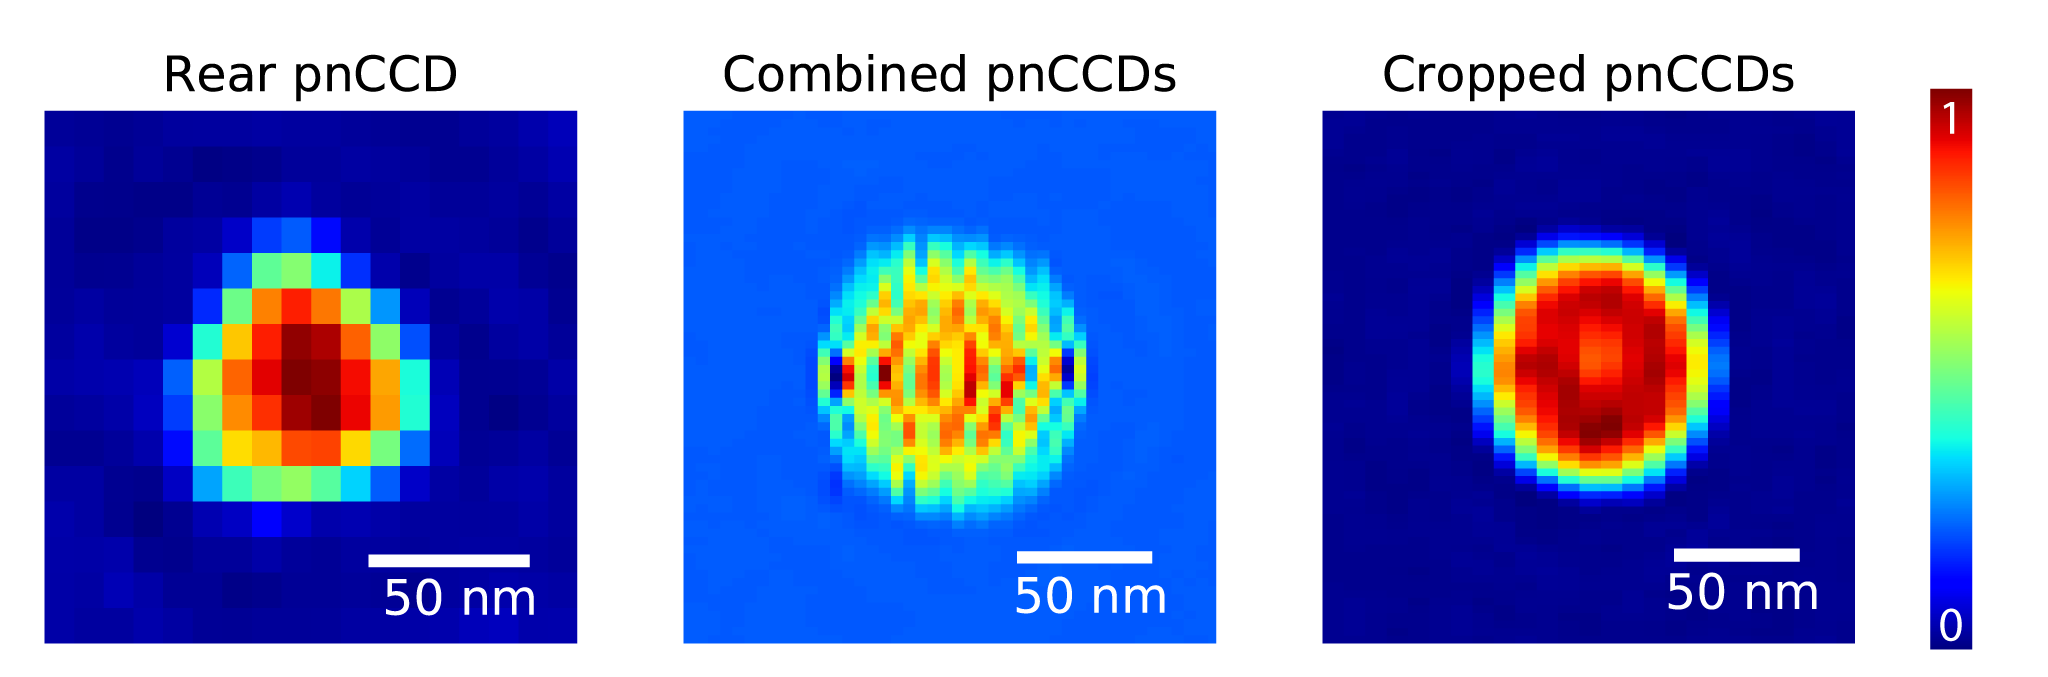
\includegraphics[width=0.95\linewidth]{images/Phase-retrieval-image.png}\\
   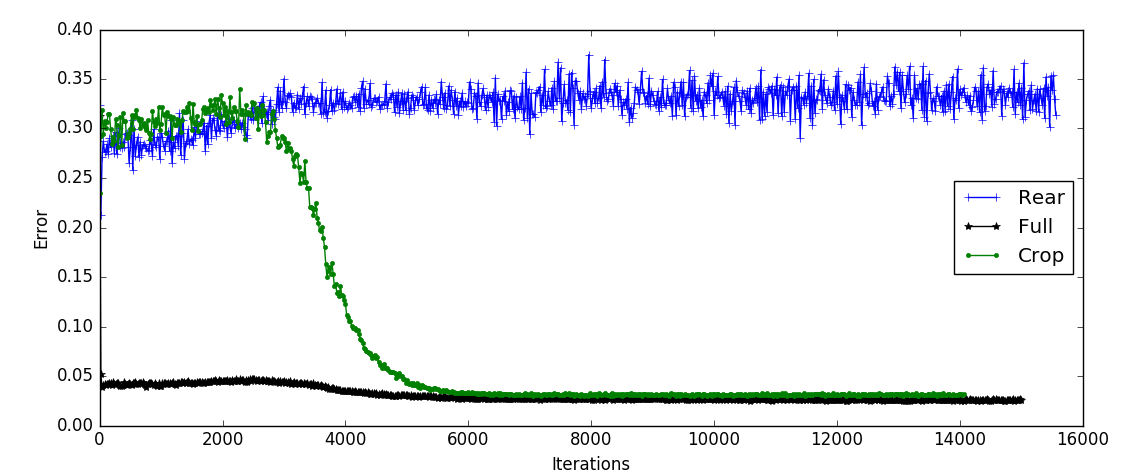
\includegraphics[height=2.5cm]{images/Phase-retrieval-error.png}
    \caption{A set of reconstructions of Xe-cluster yielded from the diffraction pattern in figure \ref{fig:ccd-image-geometry} and the corresponding real-space error over number of iterations. The real space image gathered from the rear pnCCD uses no data from the front pnCCD. This reconstruction shows a not spherical object although the density distribution appears to be reasonable for a nano-particle. The real space image reconstructed from the full front and rear pnCCD data set appears to be a spherical object but the missing areas disturb the diffraction pattern and it has become unphysical. The Xe-cluster reconstructed without the dead areas has the expected spherical shape and the density distribution appears to be physical.}
\label{fig:phase-retrieval-image}
  \end{center}
\end{figure}
While there is no consensus on how to define resolution in a coherent diffractive imaging pattern and the resulting reconstruction, there are various good estimates. A simple and conservative method to define resolution in a diffraction pattern is Abbe's criterion, which comes from microscopy and calculates the minimal resolvable feature size in a diffraction pattern. The fundamental limit that the minimal resolvable feature size is depended on the wavelength has also given us the inspiration to build short-wavelength machines such as the free electron laser and synchrotron light sources in the first place. In the far field, Abbe's criterion can be written down as
% Internal note, Max did check that we are in the far field.
\begin{equation}
    d = \frac{\lambda}{2n \sin(\frac{\Theta}{2})},
\end{equation}
with the minimal resolvable feature size $d$, the wavelength of the x-rays $\lambda$, the refractive index $n$ and the half scattering angle $\frac{\Theta}{2}$. The scattering angle is restricted by either the active detector area, which goes back to the typical understanding of a numerical aperture, or the signal intensity up to certain angles, which is in interplay with the photon wavelength. This interplay leads to the assessment that very high energy photons, e.g. $8$ keV photons that are commonly used for crystallographic purposes, scatter too little signal and too narrow scattering angles. As current results indicate, using $1-5$ keV photons ultimately leads to higher resolution images than using $8$ keV photons. TBD
%Anyway, in the 'Cropped pnCCDs' reconstruction, the experimental parameters would be $\lambda = 1.5$ nm, $n = 1$ and $\Theta = 9.3$°, hence a resolution of $3.2$ nm. Using Abbe's criterion, the 'Rear pnCCD' real space image has resolution of $4.2$ nm, which doesn't appear to make a significant difference. This is odd because judging from the reconstructions, there should be an improvement. So, let us investigate this further by translating the reconstructed pixel size into real space.
In the far field, we can use the following equation to investigate the pixel size \cite{Williams-2010-NJP}
\begin{equation}
    \Delta_{s} = \frac{\lambda L}{N \Delta_{d}},
\label{eq:relation-pixel-fourier}
\end{equation}
$L$ being the length from the interaction region to the detector, $\Delta_{i}$ being the linear pixel size that is linked to each other through the discrete Fourier transformation and $N$ being the side length of the discrete detector array. For the 'Cropped pnCCDs' reconstruction the real-space size per pixel is then $1.8 \times 0.6$ nm and for the 'Rear pnCCD' reconstruction it is $2.4 \times 2$ nm in $x \times y$, respectively. Along the y-axis there is a significant improvement that seems to be necessary for a successful reconstruction.
%
%
%
\subsection{1D reconstructions}
- Describe my algorithm in 1D in detail
%%%
%\section{Signal on time of flight detector}
%- Explain what we see in Xe, He and XeHe sample environments.\\
%- and further analysis aspects, e.g. Aqiris / psana interface.
%%%
%\section{Summary of methods}
%- Comprehensive summary 